\scanpage{146}
\mspage{20}
\unsure{premiere|première} formule \inserted{3.\unsure{9|8}.bis}, notons que l'on a égalité lorsque $M$ est la catégorie des couples $(A,B)$, $A$ un ensemble et $B$ une partie de $A$, avec les flèches évidentes, et qu'on définit $M^\pi$ (pour $\pi\ge\unsure{\aleph_0|\pi_0}$) comme la sous-catégorie str. pleine \unsure{formée|fermée} des $(A,B)$ tels que $\mathrm{card}\,A\ge\deleted{\unsure{\aleph_0}}\pi$.

\uline{Démonstration de 3.1.} Prouvons d'abord la formule 3.8.
\[
\mathrm{card}\,\mathrm{Hom}(A,X)\le s^{(r^{\pi_0})}\qquad
\left\{\begin{aligned}
&\text{si }A\in\mathrm{Filt}^r,\ X\in\mathrm{Filt}^s\\
&r\ge\deleted{\unsure{\mathrm{Sup}(}}\pi_1,\deleted{\unsure{C_1}}),\ s\ge\mathrm{Sup}(\deleted{\unsure{\pi_0|2}}\pi_1,C_1)
\end{aligned}\right.
\]
(NB. \unsure{Je n'utiliserai|Je n'utilise} pas $r\ge C_1$, postulé dans 3.1 \uline{1°})
\deleted{\unsure{Soit} $\pi_1'=\mathrm{Sup}(\pi_0,\pi_1)$.}
\deleted{\unsure{J'écris|Il est}}
\[
\begin{aligned}
A&=\varinjlim_I A_i,\qquad\mathrm{card}\,I\le r^{\pi_0},\quad A_i\in\mathrm{Filt}^{\pi_0}\\
X&=\varinjlim_J X_j\qquad\mathrm{card}\,J\le s^{\pi_1^{\deleted{\unsure{\prime|*}}}},\quad X_j\in\mathrm{Filt}^{\pi_1^{\deleted{\unsure{\prime|*}}}}\\
&\hspace{70pt}J\text{ grand devant }\pi_1^{\deleted{\unsure{\prime|*}}},\ \deleted{\text{\unsure{plus grand|donc grand} devant }\pi}
\end{aligned}
\]
On a
\[
\mathrm{Hom}(A,X\unsure{]|)}=\varprojlim_{\unsure{i|j}\in I}
\underbrace{\mathrm{Hom}(A_i,\varinjlim_J X_j)}_{
\begin{gathered}
\unsure{\Vert|\wr}\longrightarrow
\begin{gathered}\text{car les }\unsure{A|A_i}\in\mathrm{Filt}^{\pi_0}\\\text{sont }\pi_1\text{-accessibles\unsure{;|,}}\end{gathered}\\
\varinjlim_{j\in J}\underbrace{\mathrm{Hom}(A_i,X_j)}_{\text{de cardinal }\le C_1}
\end{gathered}}
\]
donc pour $\unsure{A|\forall|\text{tt}}\ i\in I$
\[
\mathrm{Hom}(A_i,X\unsure{]|)}\le\mathrm{card}(J)\times C_1\le s^{\pi_1}\times C_1=s^{\pi_1}
\]
\margin{car $s\ge C_1$ donc $s^{\pi_1}\ge C_1$}
d'où
\[
\mathrm{card}\left(\varprojlim_{j\in I}\mathrm{Hom}(A_i,X\unsure{]|)}\right)
\le (s^{\pi_1})^{\mathrm{card}\,I}\le
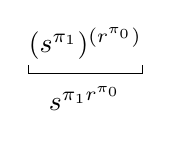
\begin{tikzpicture}[baseline=(F.base)]
\node[inner sep=0pt] (F) {$(s^{\pi_1})^{(r^{\pi_0})}$};
\draw ([yshift=-2pt]F.south west) -- ++(0,-3pt) -| ([yshift=-2pt]F.south east);
\node[below=6pt] at (F.south) {$s^{\pi_1r^{\pi_0}}$};
\end{tikzpicture}
\]
Comme $r\ge\pi_1$, on a $r^{\pi_0}\ge\pi_1$, donc $r^{\pi_0}\pi_1=r^{\pi_0}$, d'où
\[
\mathrm{card}\,\mathrm{Hom}(A,X)\le s^{(r^{\pi_0})},
\]
c'est bien la formule 3.8. Pour en tirer une estimation pour $M^r_{/X}$ (avec $X\in\mathrm{Filt}^s$),
% archive sheet number: 145
